
\section{Halbleiter}

\subsection*{p-n Übergang}
\textbf{Dotierung:} Dotierung ist das gezielte Einbringen von Störstellen bei der Züchtung des Halbleiterkristalls. Besondere technische Relevanz besitzen Störstellen mit einem Bindungselektron mehr oder weniger als das zu ersetzende Wirtsgitteratom. In der Praxis sind Dotierungskonzentrationen von etwa $10^{14}$ bis $10^{20}\si{\per\centi\meter\cubic}$, je nach Substanz, üblich. \
\textbf{Donatoren:} Donatoren besitzen ein Bindungselektron \emph{mehr} als das Wirtsgitteratom. Ein Beispiel für das beliebte Silizium ist Phosphor. Silizium besitzt 4 Valenzelektronen, während Phosphor als Teil der 5. Hauptgruppe 5 hat. Dieses fünfte Elektron wird zur chemischen Bindung im Kristallgitter nicht benötigt und kann sich so durch den Halbleiter bewegen. Es unterliegt allerdings trotzdem noch der Coulomb-Anziehung durch die nicht abgesättigte Ladung des Atomkerns. \\
\textbf{Akzeptoren:} Akzeptoren besitzen ein Bindungselektron \emph{weniger} als das zu ersetzende Wirtsgitteratom. Das fehlende Valenzelektron, das zur Bindung aber nötig ist, wird durch ein Loch ausgeglichen. Somit ist weiterhin Neutralität gewährleistet. Das Loch bewegt sich - wie das Elektron beim Donator - im Coulomb-Feld der gegenüber dem Wirtsgitteratom negativen Kernladung. Ein Beispiel eines Akzeptoren für Silizium ist das 3 wertige Bor.\\
\textbf{Isoelektronische Störstellen:} In einigen wenigen Fällen sind auch Störstellen durch gleichwertige Fremdatome von Bedeutung. Dies nennt man \emph{isoelektronische Störstellen}. So werden zwar keine zusätzlichen Ladungsträger eingebracht, doch die optischen Eigenschaften können von Interesse sein. Ein Beispiel ist das Stickstoff in GaP-Lumineszenzdioden, die das intensive grüne Leuchten verantworten.\\
\newpage
\textbf{pn-Übergang:} Bringt man p- und n-dotierte Halbleiter nun in Kontakt, so entsteht an der Kontaktstelle des dotierten Materials der \emph{pn-Übergang}. Im akzeptordotierten Bereich sind die beweglichen Ladungsträger Löcher (p-Leitung), im donatordotierten Elektronen (n-Leitung). An der Übergangsstelle können beide Sorten rekombinieren, sodass dieses Gebiet keine beweglichen Ladungsträger mehr aufweist. Dieses Gebiet, in welchem nur noch die Raumladung der Störstellenrümpfe vorhanden ist, wird Raumladungszone genannt. Die Änderung der Elektronen- bzw. Löcherkonzentration in dieser Zone führt zu einem Diffusionsstrom in diese Gebiete hinein. Dieser wird durch einen gleich großen, entgegengesetzt gerichteten Feldstrom kompensiert, sodass insgesamt ein Gleichgewicht herrscht. (siehe Skizze \ref{pn} auf Seite \pageref{pn})
\begin{figure}[htb]
	\centering
	\includegraphics[width=0.7\textwidth]{Abb/pn.eps}
	\caption{\textbf{pn-Übergang:} \emph{Quadrate:} unbewegliche Rümpfe der Donatoren/Akzeptoren. \emph{Kreise:} bewegliche Ladungsträger (Elektronen und Löcher)}
	\label{pn}
\end{figure}

\subsection*{Halbleitermaterialien}
Die Bandbreite technisch genutzter Halbleitermaterialien ist groß. Je nach Verwendungszweck und Budget kommen viele verschiedene Kristalle zum Einsatz.\\
\emph{Silizium} ist der bekannteste Halbleiter. Die größten Vorteile sind die niedrigen Kosten und die hohe Verfügbarkeit. Für Mikroprozessoren wird Silizium mit Bor (III) und Arsen (V) dotiert. Auch für Solarzellen wird einerseits das kristalline Silizium gerne eingesetzt, andererseits allerdings auch amorphes Silizium (a-Si). Hier bildet sich kein Kristallgitter aus, sondern eine glasartige Struktur. So bleiben manche Si-Bindungen frei und Wasserstoffatome können sich festsetzen. So gibt es auch innerhalb des Gaps noch erlaubte Zustände und es bilden sich keine scharfen Bandkanten aus. \label{halbmat}

\subsection*{Bestimmung der Gap-Energie}
Die Gap-Energie kann gemessen werden, indem man den Widerstand eines hochreinen Halbleiters misst, während man diesen mit Photonen unterschiedlicher Wellenlänge bestrahlt. Ab einer bestimmten materialabhängigen Wellenlänge sinkt der Widerstand sprungartig. Photonen dieser Wellenlänge haben mindestens die Gap-Energie.

\subsection*{Diffusionslänge}
Die Diffusionslänge gibt die durchschnittliche Strecke an, die ein Elektron-Loch-Paar zurücklegt, bevor es rekombiniert. 

\subsection*{Gleichrichter}
Wird die Diode in Durchlassrichtung gepolt, baut sich die Verarmungszone ab, bis die Diode ab einer kleinen materialabhängigen Grenzspannung sehr gut leitend wird. Siehe hierzu die Kennlinie einer Diode, Abb. \ref{diodekenn}.
\begin{figure}[htb]
	\centering
	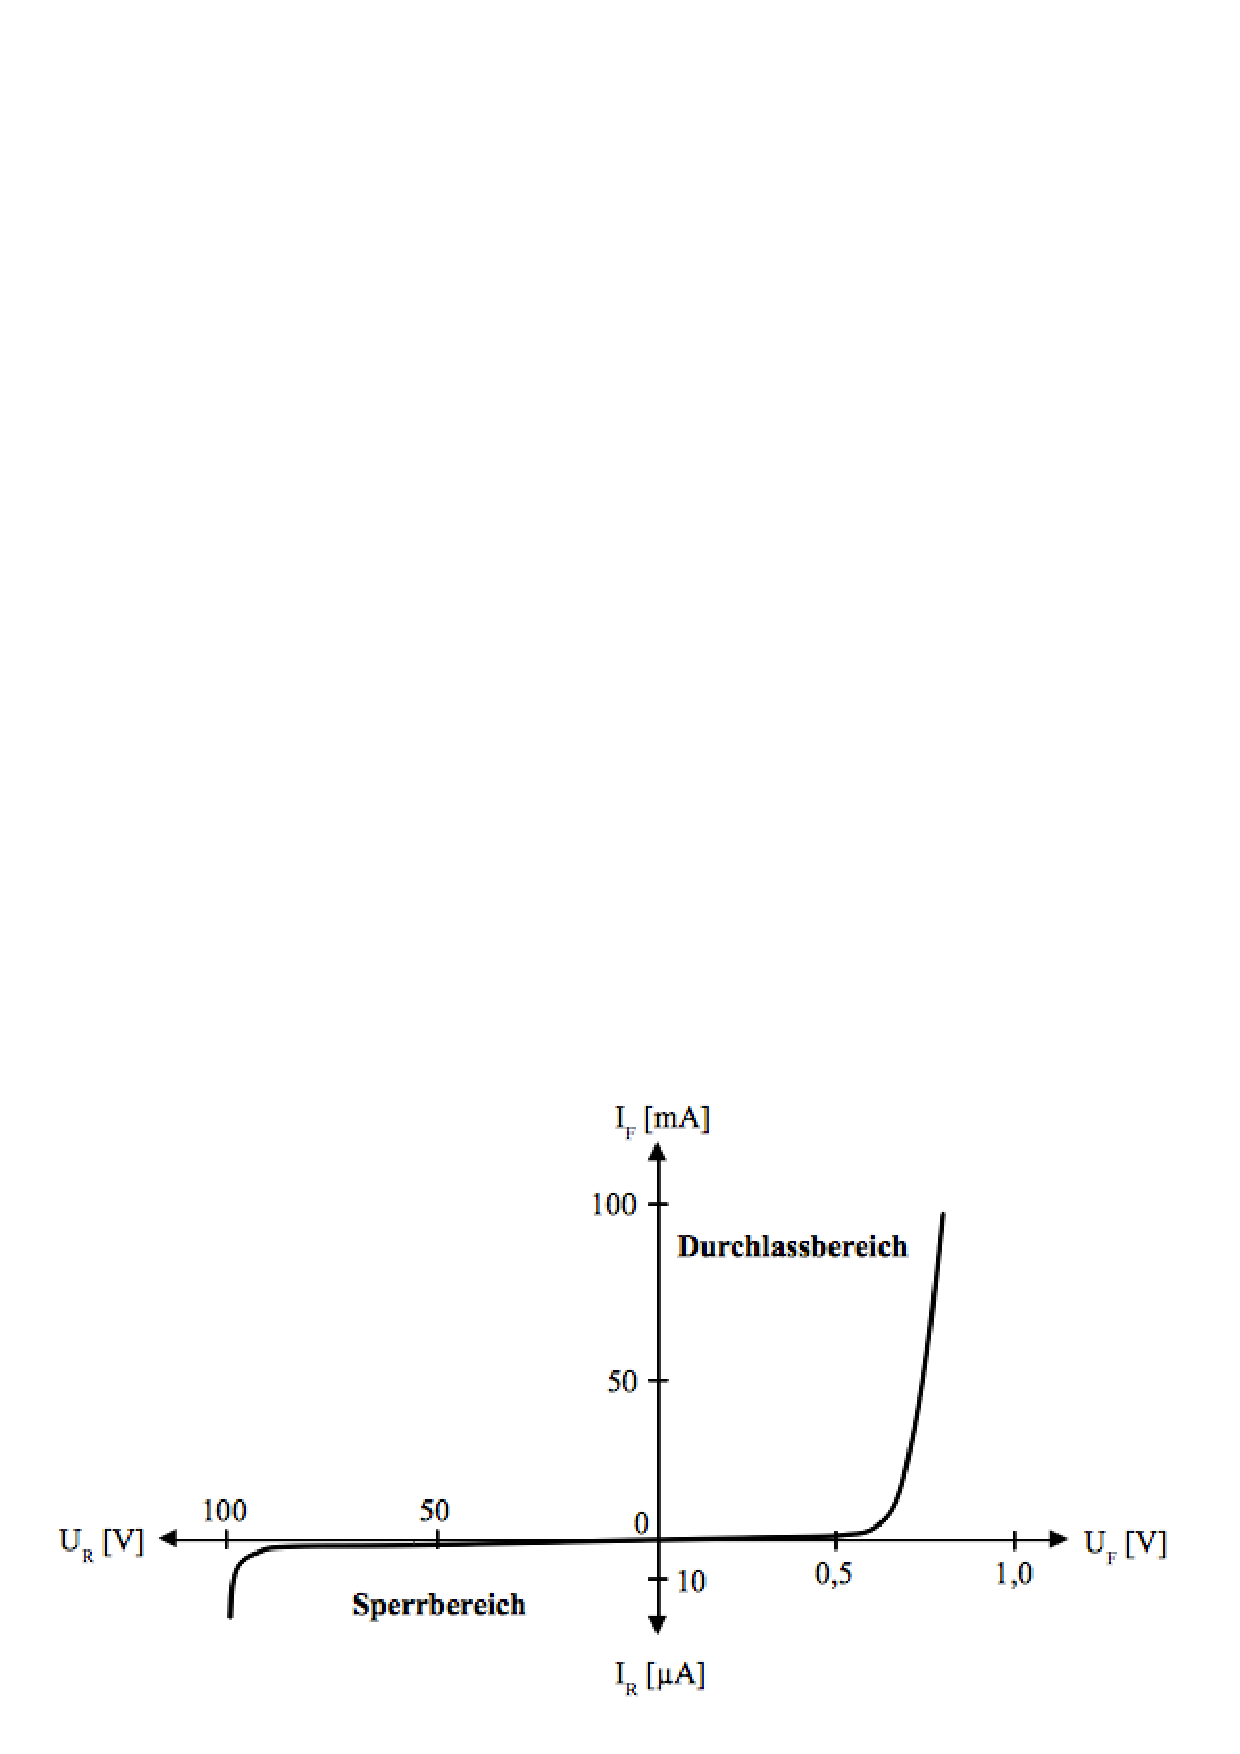
\includegraphics[width=0.8\textwidth]{Abb/Diodenkennlinie.png}
	\caption{I/U-Kennlinie einer Diode}
	\label{diodekenn}
\end{figure}


\subsection*{Temperaturabhängigkeit der I/U-Kennlinie}
Abb. \ref{kenntemp} zeigt die Temperaturabhängigkeit der I/U-Kennlinie.
\begin{figure}[htb]
	\centering
	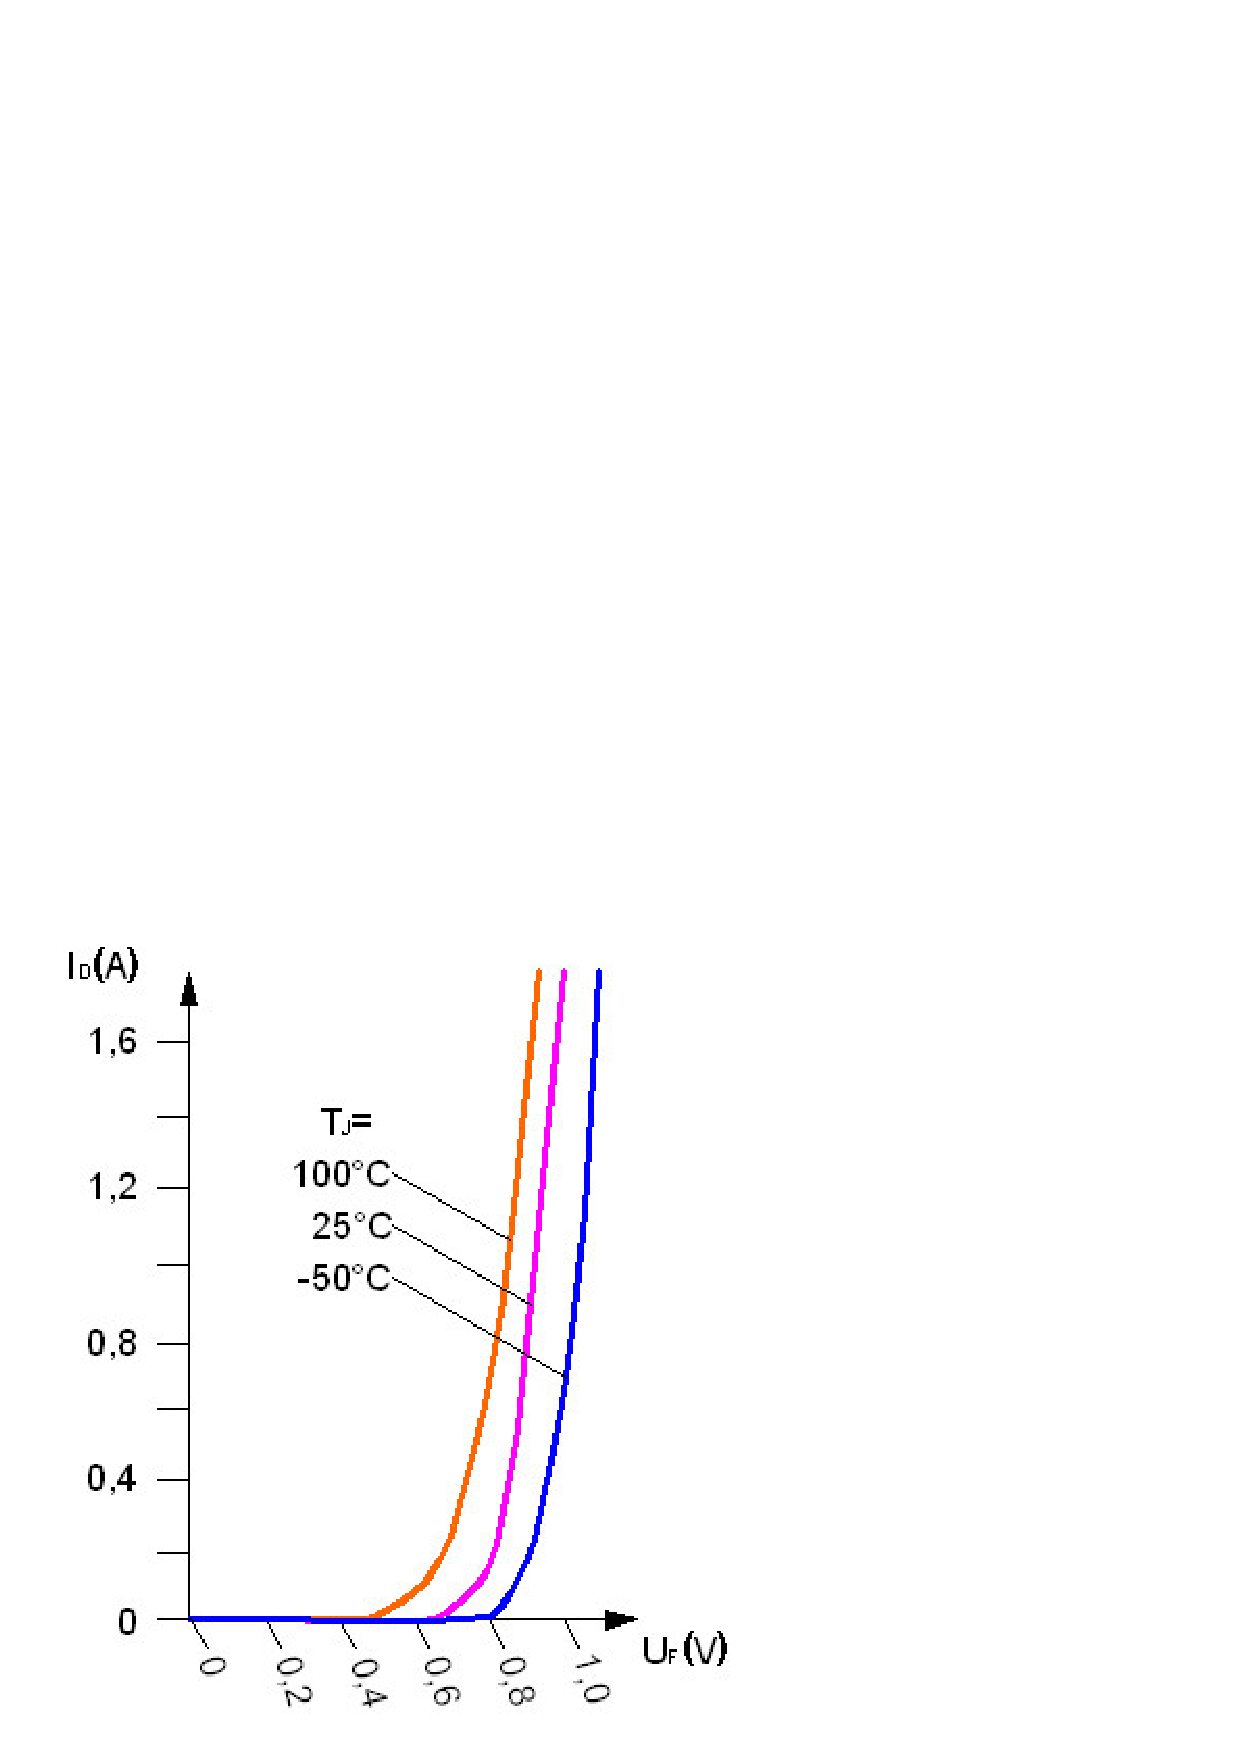
\includegraphics[width=0.4\textwidth]{Abb/diodekenn_temp.jpg}
	\caption{Kennlinie bei verschiedenen Temperaturen}
	\label{kenntemp}
\end{figure}
